% !TeX spellcheck = en_GB
% !TeX program = pdflatex
%
%

\documentclass[11pt, a4paper]{article}

\usepackage[T1]{fontenc}
\usepackage[utf8]{inputenc}
\usepackage[british]{babel}
\usepackage[left = 0mm, right = 0mm, top = 0mm, bottom = 0mm]{geometry}
\usepackage[stretch = 25, shrink = 25, tracking=true, letterspace=30]{microtype}
\usepackage{graphicx}
\usepackage{xcolor}
\usepackage{marvosym}

\usepackage{enumitem}
\setlist{parsep = 0pt, topsep = 0pt, partopsep = 1pt, itemsep = 1pt, leftmargin = 6mm}

\usepackage{FiraSans}
\renewcommand{\familydefault}{\sfdefault}

%\definecolor{cvblue}{HTML}{304263}
% \definecolor{cvblue}{HTML}{4A4E5A}
\definecolor{cvblue}{HTML}{373737}

%%%%%%% USER COMMAND DEFINITIONS %%%%%%%%%%%%%%%%%%%%%%%%%%%
\newcommand{\dates}[1]{\hfill\mbox{\textbf{#1}}}
\newcommand{\is}{\par\vskip.5ex plus .4ex}
%\newcommand{\smaller}[1]{{\small$\diamond$\ #1}}
\newcommand{\smaller}[1]{{\small-\ #1}}
\newcommand{\headleft}[1]{\vspace*{3ex}\textsc{\textbf{#1}}\par%
    \vspace*{-1.5ex}\hrulefill\par\vspace*{0.7ex}}
\newcommand{\headright}[1]{\vspace*{2.5ex}\textsc{\Large\color{cvblue}#1}\par%
     \vspace*{-2ex}{\color{cvblue}\hrulefill}\par}
%%%%%%%%%%%%%%%%%%%%%%%%%%%%%%%%%%%%%%%%%%%%%%%%%%%%%%%%%%%%

\usepackage[colorlinks = true, urlcolor = white, linkcolor = white]{hyperref}

\begin{document}

\setlength{\topskip}{0pt}
\setlength{\parindent}{0pt}
\setlength{\parskip}{0pt}
\setlength{\fboxsep}{0pt}
\pagestyle{empty}
\raggedbottom

\begin{minipage}[t]{0.33\textwidth} %% Left column
\colorbox{cvblue}{\begin{minipage}[t][5mm][t]{\textwidth}\null\hfill\null\end{minipage}}

\vspace{-.2ex}
\colorbox{cvblue!90}{\color{white}  %% LEFT BOX
\kern0.09\textwidth\relax
\begin{minipage}[t][293mm][t]{0.82\textwidth}
\raggedright
\vspace*{2.5ex}

\Large Anatolii \textbf{\textsc{Storchak}} \normalsize

\null\hfill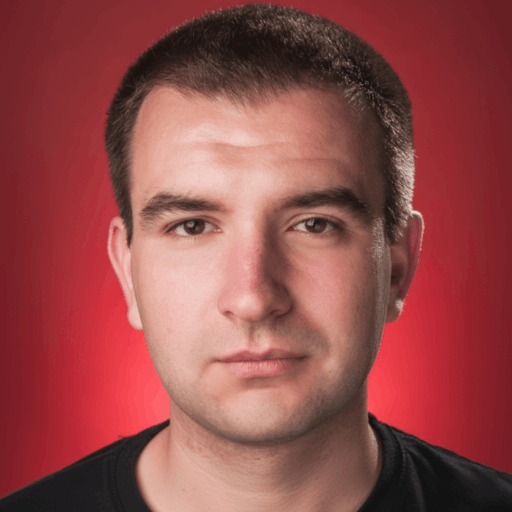
\includegraphics[width=0.65\textwidth]{my_photo.png}\hfill\null

\vspace*{0.5ex}

\headleft{Profile}
Engineer with strong leadership qualities, clear vision and a results-oriented mindset. I can work effectively under pressure, adapt quickly to unexpected changes, and find solutions in critical situations.

\headleft{Languages}
\textbf{English}~(Upper-Intermediate+) \\[0.5ex]
\textbf{Ukrainian}~(native)

\headleft{Certificates \& Courses}
\textsc{Machine Learning} \\[0.3ex]
\textit{Stanford University / Coursera} \\[0.3ex]
Issued Jun 2022 \\[0.3ex]
{\small Credential ID: \texttt{2LAD3QSM5YP2}}

% \vfill

\headleft{Contact}
\small
% \MVAt\
{\small gumbygm0@gmail.com} \\[0.4ex]
\phantom{x}
\normalsize


\end{minipage}%
\kern0.09\textwidth\relax
}
\end{minipage}% Right column
\hskip2.5em
\begin{minipage}[t]{0.56\textwidth}
\setlength{\parskip}{0.8ex}

\vspace{2ex}

\headright{Skills}

\smaller{Software development for microcontrollers using Embedded C/C++, and application-level products in Javascript, Python, Golang.}

\is
\smaller{Data visualisation and statistical processing tools: MATLAB, Python (SciPy, Matplotlib, Keras, PyTorch).}

\is
\smaller{Basic knowledge of CAD systems for 3D modelling and design of electrical schematics and PCBs.}

\is
\smaller{2D animation (Javascript Canvas), web applications and microservices.}


\headright{Experience}

\textsc{UAV Systems Engineer} --- \textit{UAV Equipment & Tools Projects.} \dates{2023--2026} \\
\smaller{RnD, Project management, Software development, CAD modeling and PCB design participation.}

\is
\textsc{Lead Software Engineer} at \textit{Liniad.} \dates{2020.12--2026} \\
\smaller{Development of company platform for modification and analytics of interactive advertising on React and Node.js.} \\
\smaller{Setting up development and CI/CD integration processes for the interactive and gaming advertising department.} \\
\smaller{Development of interactive advertising (HTML5 canvas, Javascript).}

\is
\textsc{Software Engineer} at \textit{Titanium Labs.} \dates{2018.08--2020.11} \\
\smaller{Development of interactive game advertising (HTML5 canvas, Javascript).} \\
\smaller{Building web applications.} \\
\smaller{Leading a small team, mentoring junior developers.}

\is
\textsc{Software Engineer} at \textit{TopLab --- IoT for startups.} \dates{2018.01--2018.08} \\
\smaller{Embedded C/C++ programming for devices with inertial navigation systems (IMU) and Bluetooth LE.} \\
\smaller{Development and reverse engineering of device communication protocols over CAN and RS485 buses.} \\
\smaller{Creating Linux distributions for embedded systems using Yocto and Armbian build systems.}

\is
\textsc{Automotive Electrician.} \dates{2017.06--2018.01} \\
\smaller{Diagnostics and repair of electrical systems of cars and buses.}


\headright{Education}

\textsc{PhD --- Doctor of Philosophy.} Metrology and Information-Measuring Systems. \\
\textit{Cherkasy State Technological University.} \dates{2018--2025}

\is
\textsc{MSc --- Master of Science.} Instrumentation and Robotics. \\
\textit{Cherkasy State Technological University.} \dates{2014--2018}

\is
\textsc{Associate Degree.} Diagnostics and Repair of Electrical Equipment of Automobiles and Tractors. \textit{Cherkasy Polytechnic College.} \dates{2010--2014}


\headright{Interests}

Robotics \quad$\cdot$\quad Machine Learning \quad$\cdot$\quad Electronic devices \quad$\cdot$\quad Automotive industry

\end{minipage}

\end{document}
